\chapter{Additional data from five SCLC patients}
\label{app.sclc}

\begin{figure}[p]
    \centering
    \begin{subfigure}{0.6\textwidth}
        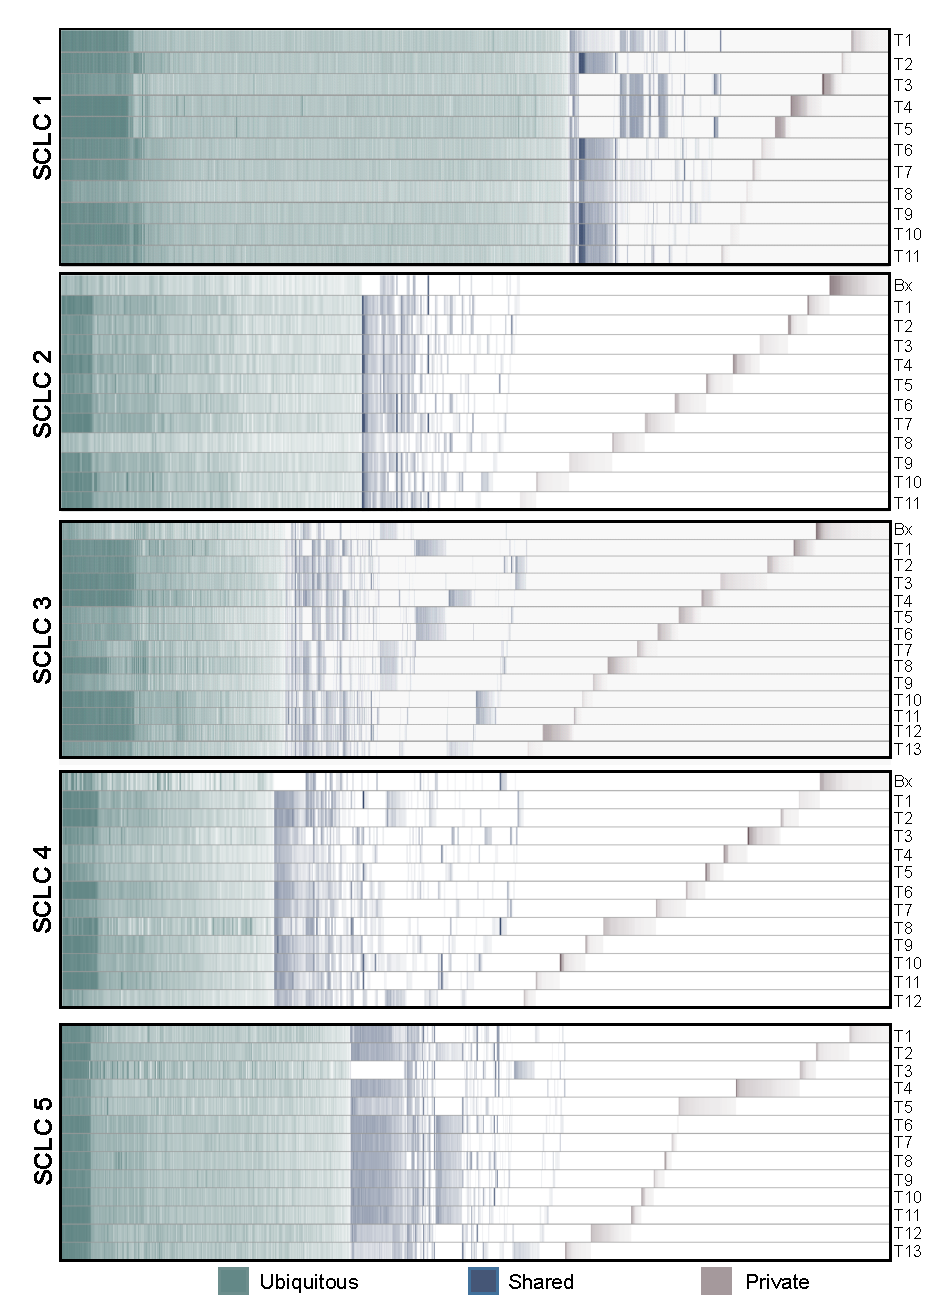
\includegraphics[width=\linewidth,keepaspectratio]{images/sclc/mutation_heatmap}
        \caption{}\label{fig:sclc:mutation_heatmaps}
    \end{subfigure}
    
    \begin{subfigure}{\textwidth}
        \centering
        \begin{tabular}{cccccc}
            Variant Type & SCLC 1 & SCLC 2 & SCLC 3 & SCLC 4 & SCLC 5 \\
            \hline
            \# Ubiquitous & 984 & 202 & 460 & 141 & 372 \\
            \# Shared & 121 & 84 & 289 & 114 & 161 \\
            \# Private & 501 (32\%) & 270 (49\%) & 954 (56\%) & 296 (54\%) & 534 (50\%)
        \end{tabular}
        \caption{}\label{fig:sclc:clonal_mut_num}
    \end{subfigure}
    \vspace{-0.5cm}
    \caption[SNVs and indels in five SCLC patients.]{Tumor or geographic distribution of somatic variants in five SCLC autopsy patients. Somatic variants include single nucleotide variants (SNVs) and insertions/deletions (indels). (\subref{fig:sclc:mutation_heatmaps}) Heatmaps of somatic variants detected in autopsy tumor samples (T) and pre-treatment biopsy samples (Bx). Reference key in Supplemental data S1 for organ sites of tumor involvement. Variant classification is indicated by colored box key. (\subref{fig:sclc:clonal_mut_num}) Variant classification based on distribution across tumor samples in each patient. Ubiquitous: variants detected in all tumor samples, including biopsy. Shared: variants detected in a subset of tumor samples of a patient. Private: variants detected in only one tumor sample of a patient.}
    \label{fig:sclc:mutation_overview}
\end{figure}

\begin{figure}[p]
    \centering
    \hspace{1cm}%
    \begin{subfigure}{0.17\textwidth}
        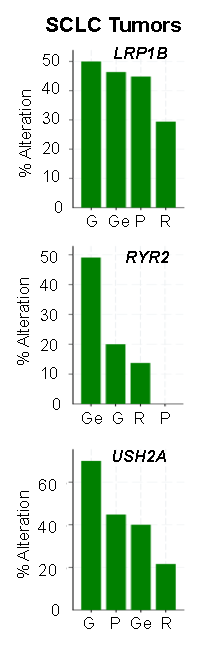
\includegraphics[width=\linewidth,keepaspectratio]{images/sclc/drivers_210}
        \caption{}\label{fig:sclc:drivers_210}
    \end{subfigure}%
    \hfill%
    \begin{subfigure}{0.73\textwidth}
        \includegraphics[width=\linewidth,keepaspectratio]{images/sclc/drivers_cbioportal}
        \caption{}\label{fig:sclc:drivers_cbioportal}
    \end{subfigure}%
    \hspace{1cm}
    
    \caption[Prevalence of \textit{LRP1B}, \textit{RYR2} and \textit{USH2A} mutations.]{(\subref{fig:sclc:drivers_210}) Bar graphs generated through cBioPortal for Cancer Genomics demonstrating frequency of genomic alterations in \textit{LRP1B}, \textit{RYR2}, and \textit{USH2A} in four additional SCLC datasets containing a total of 210 tumor samples (predominantly primary SCLC)\@. G, Gardner \textit{et al} \cite{gardner2017}, n=20; Ge, George \textit{et al} \cite{george2015}, n=110; P, Peifer \textit{et al} \cite{peifer2012}, n=29; R, Rudin \textit{et al} \cite{rudin2012}, n=51. (\subref{fig:sclc:drivers_cbioportal}) Bar graphs generated through cBioPortal for Cancer Genomics demonstrating frequency of genomic alterations in \textit{LRP1B}, \textit{RYR2}, and \textit{USH2A} in 11,777 cancer samples from the TCGA Pan-Cancer Atlas studies and 210 SCLC samples (yellow arrows). Type of gene alteration is defined by the colored circle key at the bottom. The five cancer types with highest rates of genomic alterations for each gene are labeled. S, small cell lung cancer; E, endometrial carcinoma; EG, esophagogastric adenocarcinoma; ES, esophageal squamous cell carcinoma; F, fibrolamellar carcinoma. M, melanoma; N, non-small cell lung cancer.}
    \label{fig:sclc:driver_bar_graphs}
\end{figure}

\begin{figure}[p]
    \centering
    \includegraphics[width=0.9\textwidth,keepaspectratio]{images/sclc/curated_cnv_plots}
    \caption[Curated CNVs in SCLC autopsy patients.]{Curated copy number variations (CNVs) in five SCLC autopsy patients. Raw output from FALCON, an allele-specific CNV caller using next-generation sequencing data as input, was manually curated to identify discrete events of CNVs in 22 autosomes. Data from all tumor samples per patient were pooled into a composite CNV profile as shown. CNV $>2$ is considered a gain; CNV $<0.5$ a loss. Chromosome arms containing CNVs involving oncogenes and tumor suppressors are labeled. Red: copy event in major allele. Blue: copy event in minor allele. Green: no change in one or both alleles.}
    \label{fig:sclc:curated_cnv_plots}
\end{figure}

\begin{figure}[p]
    \centering
    \begin{subfigure}{\textwidth}
        \begin{tabular}{ccccc}
            \textbf{Variant in} & \textbf{Variant} & \textbf{\#Autopsy} & \textbf{\#ctDNA} & \textbf{\% SNVs detected} \\
            \textbf{\# Autopsy Tumors} & \textbf{Classification} & \textbf{SNVs} & \textbf{SNVs} & \textbf{by ctDNA} \\
            \hline
            13 tumors & Ubiquitous & 293 & 285 & 97 \\
            2--12 tumors & Shared & 194 & 125 & 64 \\
            1 tumor & Private & 292 & 9 & 3
        \end{tabular}
        \caption{}\label{fig:sclc:tissue_ctdna_snv_table}
    \end{subfigure}
    
    \vspace{0.5cm}
    \begin{subfigure}{\textwidth}
        \begin{tabular}{ccccc}
            \textbf{Variant in} & \textbf{Variant} & \textbf{\#Autopsy} & \textbf{\#ctDNA} & \textbf{\% Indel} \\
            \textbf{\# Autopsy Tumors} & \textbf{Classification} & \textbf{Indels} & \textbf{Indels} & \textbf{Concordance} \\
            \hline
            13 tumors & Ubiquitous & 13 & 13 & 100 \\
            2--12 tumors & Shared & 12 & 4 & 33 \\
            1 tumor & Private & 43 & 27 & 63
        \end{tabular}
        \caption{}\label{fig:sclc:tissue_ctdna_indel_table}
    \end{subfigure}
    
    \hspace{0.1\textwidth}%
    \begin{subfigure}{0.35\textwidth}
        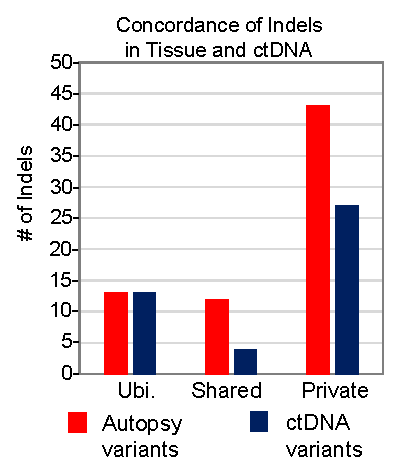
\includegraphics[width=\linewidth,keepaspectratio]{images/sclc/tissue_ctdna_concordance_indel}
        \caption{}\label{fig:sclc:tissue_ctdna_concordance_indel}
    \end{subfigure}%
    \hfill%
    \begin{subfigure}{0.38\textwidth}
        \vspace{0.1cm}
        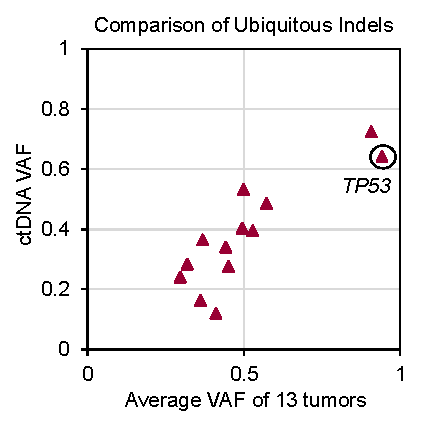
\includegraphics[width=\linewidth,keepaspectratio]{images/sclc/tissue_ctdna_ubiq_indel}
        \vspace{-0.1cm}
        \caption{}\label{fig:sclc:tissue_ctdna_ubiq_indel}
    \end{subfigure}%
    \hspace{0.1\textwidth}
    
    \caption[SNV and indel concordance in patient SCLC5 tumor tissue and ctDNA.]{Concordance of somatic variants in tumor tissues and ctDNA in patient SCLC5. (\subref{fig:sclc:tissue_ctdna_snv_table}) Summary of concordance analysis of tumor and ctDNA SNVs. (\subref{fig:sclc:tissue_ctdna_indel_table}) Summary of concordance analysis of tumor and ctDNA indels. (\subref{fig:sclc:tissue_ctdna_concordance_indel}) Bar graph showing number of indels classified as ubiquitous, shared, or private detected in tumor samples and ctDNA\@. (\subref{fig:sclc:tissue_ctdna_ubiq_indel}) The average variant allele frequency (VAF) of ubiquitous indels (including \textit{TP53}) in thirteen tumors was compared with VAF of ctDNA indels.}
    \label{fig:sclc:tissue_ctdna_concordance_detail}
\end{figure}

\begin{figure}[htbp]
    \centering
    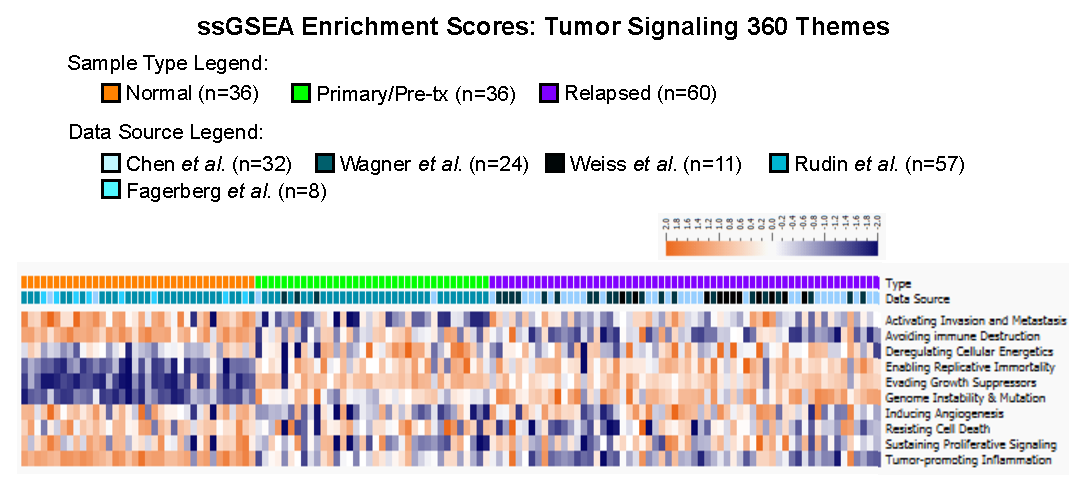
\includegraphics[width=0.84\textwidth,keepaspectratio]{images/sclc/ssgsea_heatmap}
    \caption[Heatmap of ssGSEA enrichment for 132 tissue samples.]{Heatmap of ssGSEA enrichment scores for themes in NanoString Tumor Signaling 360 in normal, primary/pre-treatment and relapsed SCLC samples. Sample type and data source are as labeled at the top of heatmap. Tumor samples had increased enrichment of genes annotated as ``enabling replicative immortality'', ``evading growth suppressors'', and ``genome instability and mutation''. Tumor samples had decreased enrichment of genes annotated as ``avoiding immune destruction'' and ``tumor-promoting inflammation''. Sample sizes are as indicated.}
    \label{fig:sclc:ssgsea_heatmap}
\end{figure}

\begin{figure}[htbp]
    \centering
    \begin{subfigure}{0.84\textwidth}
        \includegraphics[width=\linewidth,keepaspectratio]{images/sclc/ssgsea_autopsy_boxplot}
        \caption{}\label{fig:sclc:ssgsea_autopsy_boxplot}
    \end{subfigure}
    
    \begin{subfigure}{0.84\textwidth}
        \includegraphics[width=\linewidth,keepaspectratio]{images/sclc/imsig_autopsy_boxplot}
        \caption{}\label{fig:sclc:imsig_autopsy_boxplot}
    \end{subfigure}
    \vspace{-0.5cm}
    \caption[ssGSEA and ImSig scores for SCLC autopsy samples.]{(\subref{fig:sclc:ssgsea_autopsy_boxplot}) ssGSEA analysis of normal, pre-treatment and relapsed SCLC tumors from the research autopsy cohort only. (\subref{fig:sclc:imsig_autopsy_boxplot}) ImSig analysis of normal, pre-treatment and relapsed SCLC tumors from the research autopsy cohort only.}
    \label{fig:sclc:immune_rna_imsig}
\end{figure}

\begin{figure}[p]
    \centering
    \begin{subfigure}{0.25\textwidth}
        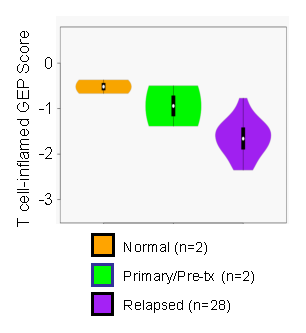
\includegraphics[width=\linewidth,keepaspectratio]{images/sclc/gep_violin_autopsy}
        \caption{}\label{fig:sclc:gep_violin_autopsy}
    \end{subfigure}
    
    \vspace{0.1cm}
    \begin{subfigure}{0.89\textwidth}
        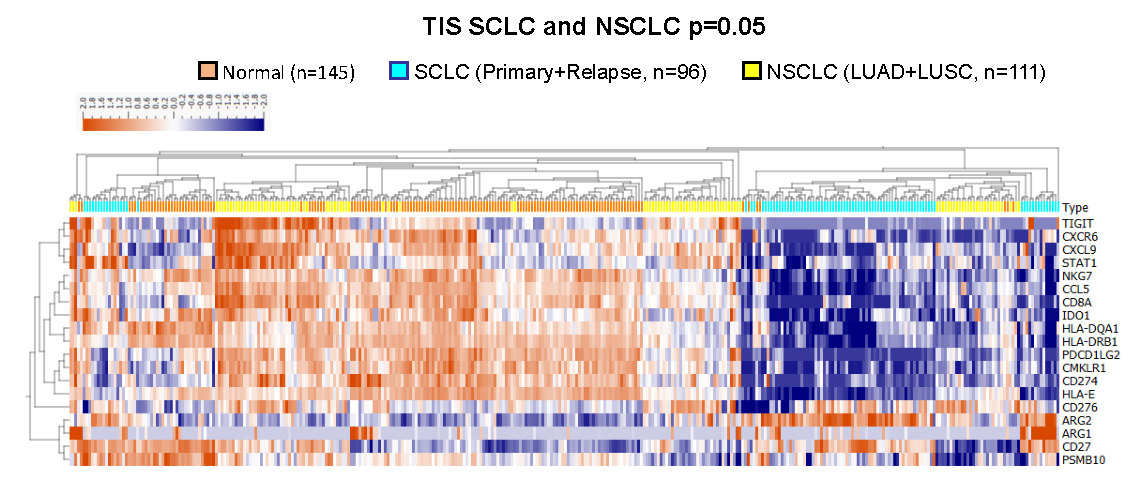
\includegraphics[width=\linewidth,keepaspectratio]{images/sclc/tis_genes_heatmap}
        \caption{}\label{fig:sclc:tis_genes_heatmap}
    \end{subfigure}
    
    \vspace{0.1cm}
    \hspace{0.05\textwidth}%
    \begin{subfigure}{0.585\textwidth}
        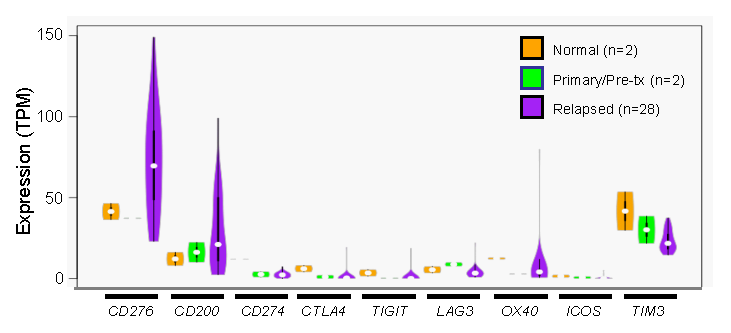
\includegraphics[width=\linewidth,keepaspectratio]{images/sclc/checkpoint_violin_autopsy}
        \caption{}\label{fig:sclc:checkpoint_violin_autopsy}
    \end{subfigure}%
    \hfill%
    \begin{subfigure}{0.265\textwidth}
        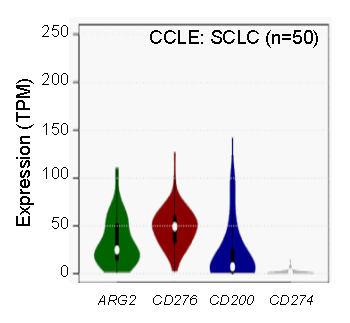
\includegraphics[width=\linewidth,keepaspectratio]{images/sclc/checkpoint_violin_ccle}
        \caption{}\label{fig:sclc:checkpoint_violin_ccle}
    \end{subfigure}%
    \hspace{0.05\textwidth}
    \vspace{-0.5cm}
    \caption[GEP scores and associated gene TPMs.]{(\subref{fig:sclc:gep_violin_autopsy}) T cell-inflamed Gene Expression Profile (GEP) scores for normal, pre-treatment and relapsed SCLC tumors from the research autopsy cohort only. (\subref{fig:sclc:tis_genes_heatmap}) Hierarchical clustering of log-transformed TPM values of T cell-inflamed GEP genes, \textit{ARG1}, and \textit{ARG2} in normal lung, SCLC, and TCGA NSCLC samples. NSCLC samples include lung adenocarcinoma (LUAD) and squamous cell carcinoma (LUSC)\@. SCLC samples include primary and relapse. Normal includes pooled normal lung samples from the SCLC and NSCLC cohorts. (\subref{fig:sclc:checkpoint_violin_autopsy}) Violin plot of TPM values of immune checkpoint genes in normal, pre-treatment and relapsed SCLC tumors from the research autopsy cohort only. (\subref{fig:sclc:checkpoint_violin_ccle}) Violin plots of TPM values of selected checkpoint genes and \textit{ARG2} in fifty SCLC cell lines from the Cancer Cell Line Encyclopedia.}
    \label{fig:sclc:gep_detail}
\end{figure}

\begin{figure}[p]
    \centering
    \includegraphics[width=0.93\textwidth,keepaspectratio]{images/sclc/classification_scatter}
    \vspace{-0.5cm}
    \caption[Relative expression of SCLC subtype-defining genes.]{Relative expression of the genes \textit{ASCL1}, \textit{NEUROD1}, \textit{YAP1}, and \textit{POU2F3}, which were used to classify SCLC tumor samples following a previously established method \cite{rudin2019} in pooled SCLC cohorts. Normal samples are excluded from this analysis. Samples are labeled by classification (colored dot), and samples marked ``unclassified'' were later manually assigned to a classification based on highest expression (TPM) of one of 4 above genes.}
    \label{fig:sclc:classification_scatter}
\end{figure}

\begin{figure}[htbp]
    \centering
    \includegraphics[width=0.9\textwidth,keepaspectratio]{images/sclc/imsig_subtype_boxplot}
    \vspace{-0.5cm}
    \caption[ImSig scores by SCLC subtype.]{Box plots of ImSig scores in the different SCLC subtypes versus normal lung for different immune cell types in the adaptive (B and T cells) and innate immune system.}
    \label{fig:sclc:imsig_subtype_boxplot}
\end{figure}
